\chapter{Theoretical Aspects}

% ----------------------------------------------------------

\section{Kolmogorov-Arnold representation theorem (KART)}

The theory behind Kolmogorov-Arnold Networks (KANs) stems from the Kolmogorov-Arnold representation theorem (KART). The KART guarantees that any continuous multivariate function can be represented as a superposition of univariate functions. This concept fundamentally underpins the design and capabilities of KANs.

Vladimir Arnold and Andrey Kolmogorov established that if $f$ is a multivariate continuous function on a bounded domain, then $f$ can be written as a finite composition of continuous functions of a single variable and the binary operation of addition. More specifically, for a smooth $f:[0,1]^n\to\mathbb{R}$,
\begin{equation}\label{eq:KART}
    f(\mathbf{x}) = f(x_1,\cdots,x_n)=\sum_{q=1}^{2n+1} \Phi_q\left(\sum_{p=1}^n\phi_{q,p}(x_p)\right),
\end{equation}
where $\phi_{q,p}:[0,1]\to\mathbb{R}$ and $\Phi_q:\mathbb{R}\to\mathbb{R}$. In a sense, they showed that the only true multivariate function is addition, since every other function can be written using univariate functions and sum. One might naively consider this great news for machine learning: learning a high-dimensional function boils down to learning a polynomial number of 1D functions. However, these 1D functions can be non-smooth and even fractal, so they may not be learnable in practice. Because of this pathological behavior, the Kolmogorov-Arnold representation theorem was basically sentenced to death in machine learning, regarded as theoretically sound but practically useless.

However, we are more optimistic about the usefulness of the Kolmogorov-Arnold theorem for machine learning. First of all, we need not stick to the original Eq.~(\ref{eq:KART}) which has only two-layer non-linearities and a small number of terms ($2n+1$) in the hidden layer: we will generalize the network to arbitrary widths and depths. Secondly, most functions in science and daily life are often smooth and have sparse  compositional structures, potentially facilitating smooth Kolmogorov-Arnold representations. The philosophy here is close to the mindset of physicists, who often care more about typical cases rather than worst cases. After all, our physical world and machine learning tasks must have structures to make physics and machine learning useful or generalizable at all.

\section{Theoretical Explanation}

The KART, in its original form, posits a specific two-layer structure with a fixed width:
\begin{itemize}
    \item Input Layer: Takes an n-dimensional input vector.
    \item Hidden Layer: Consists of 2n+1 neurons.
    \item Output Layer: Produces a scalar output.
\end{itemize}

\begin{figure}[t]
    \centering
    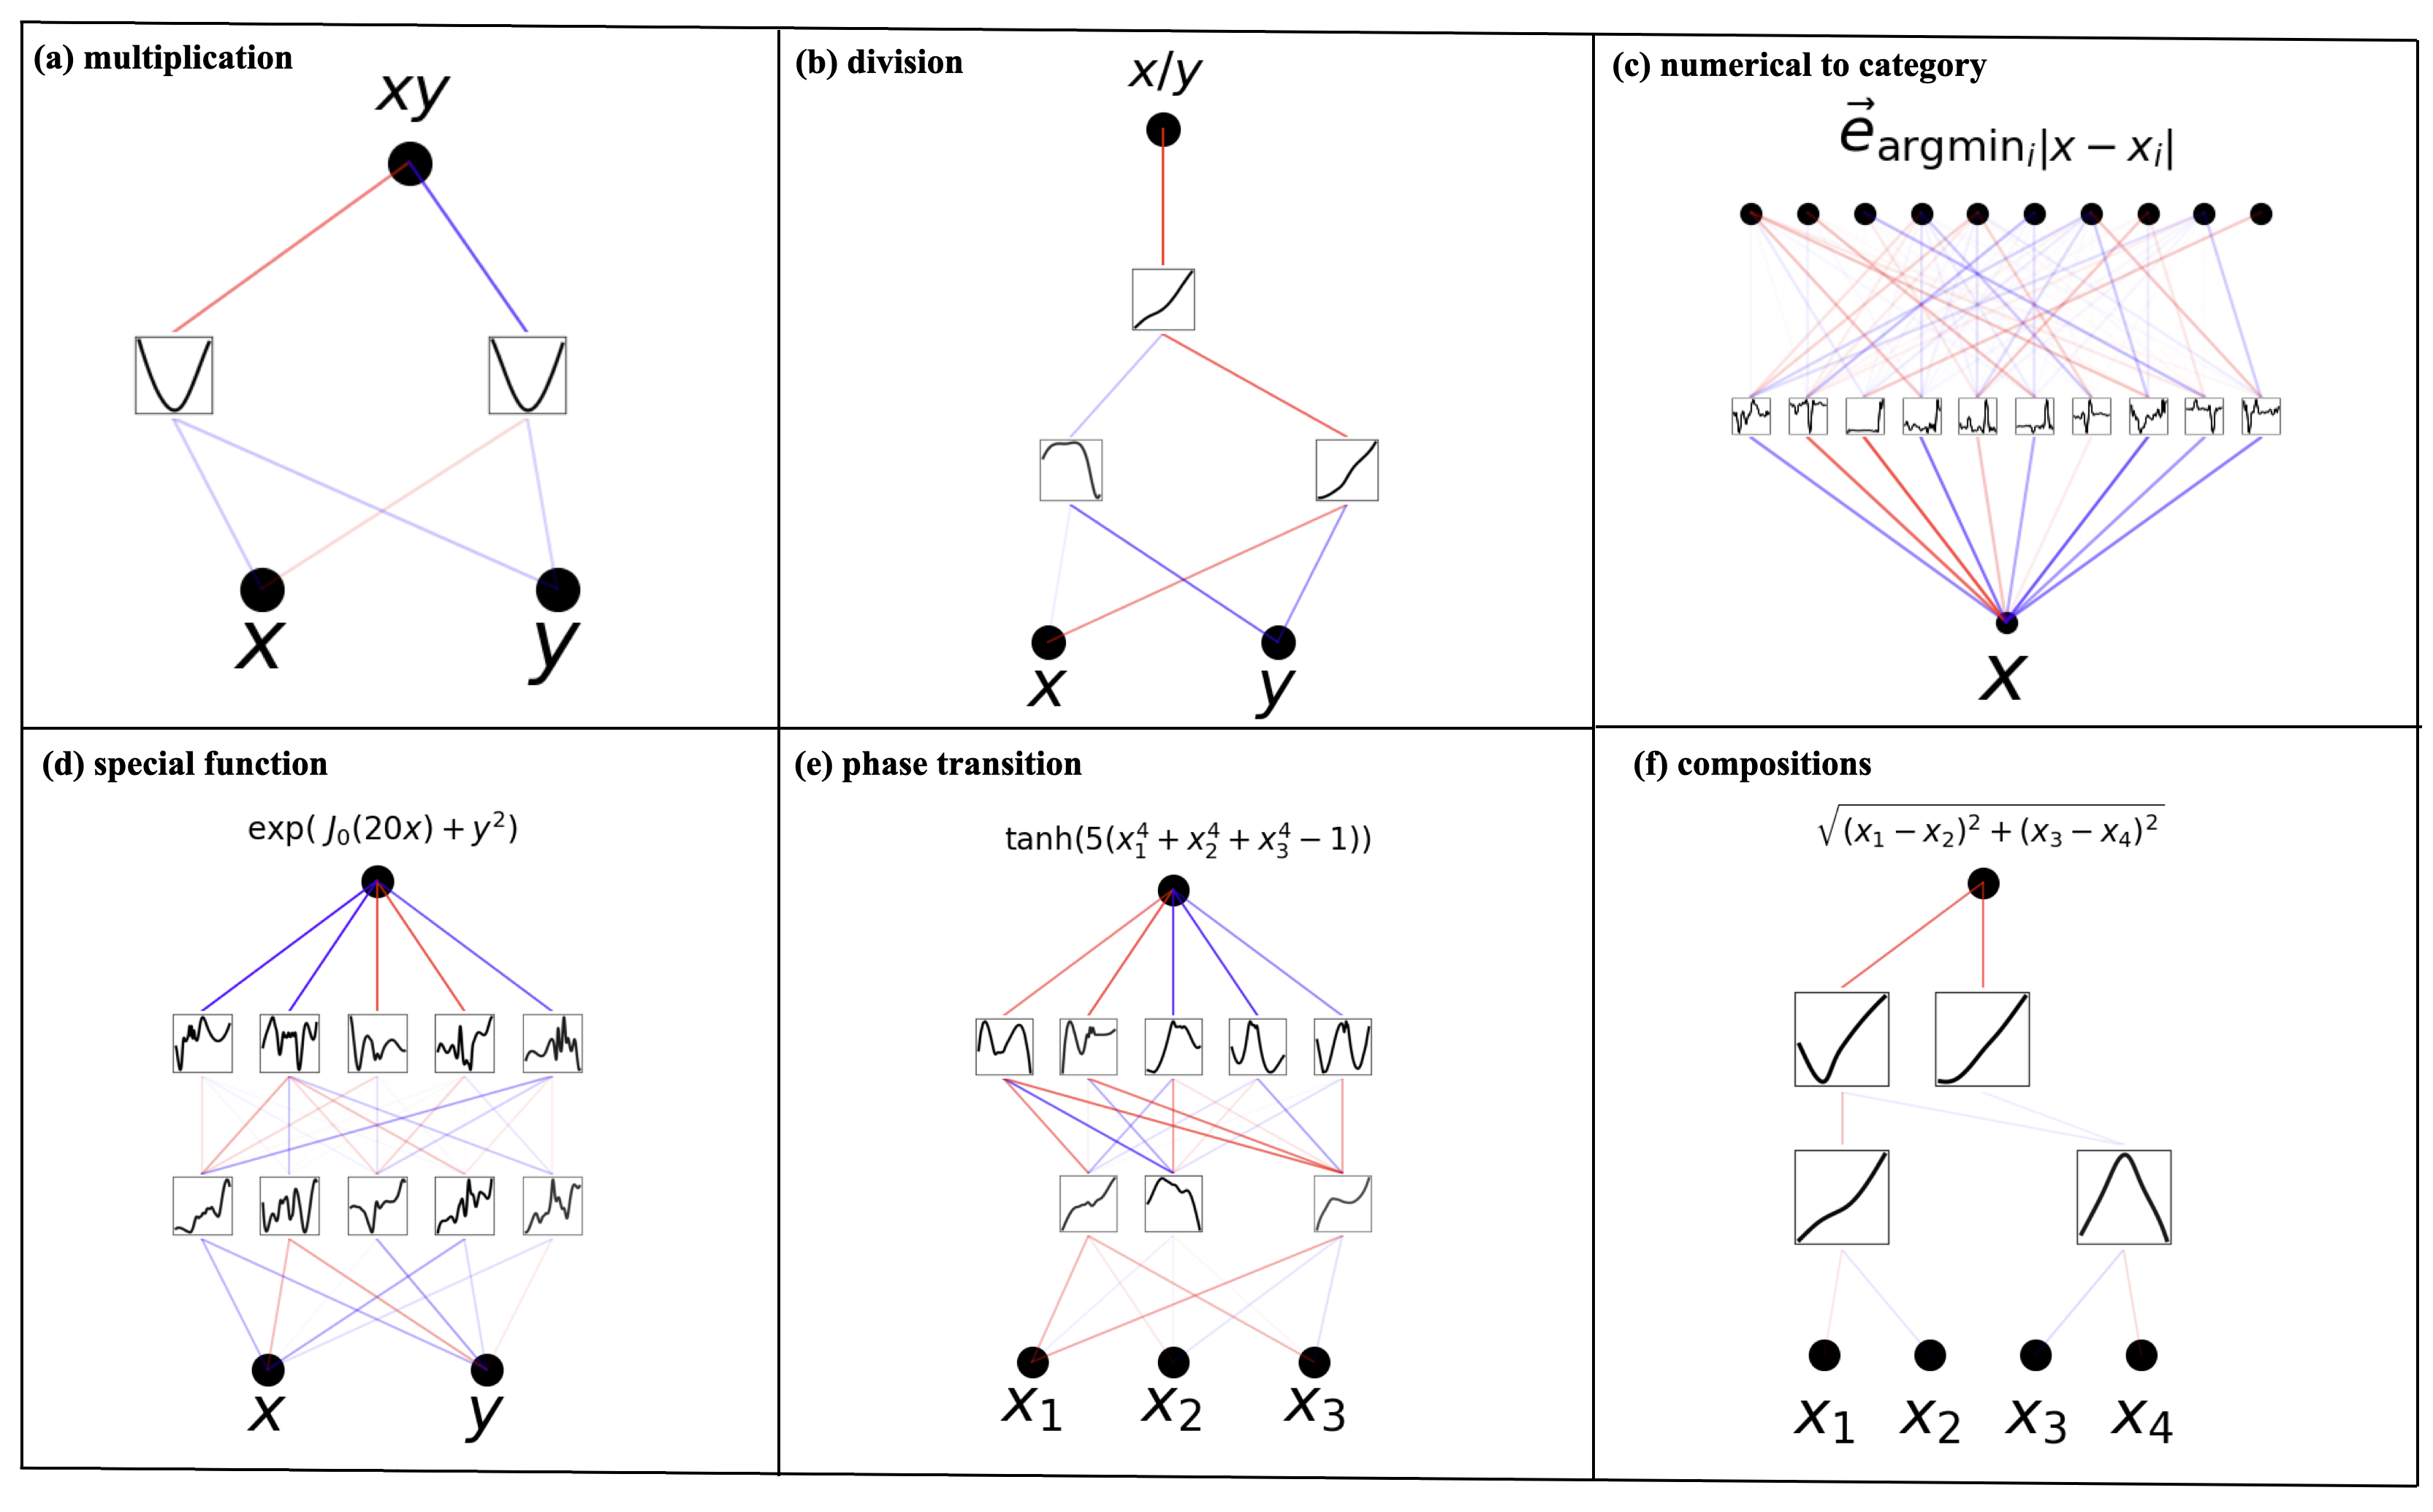
\includegraphics[width=0.9\linewidth]{Images/lan_interpretable_examples.png}
    \caption{LANs on synthetic examples. LANs do not appear to be very interpretable.}
    \label{fig:lan-interpretable-examples}
\end{figure}

The hidden layer implements a set of inner functions, each operating on a single input dimension. These inner functions are then combined by outer functions to produce the final output.
However, KANs extend this theoretical foundation by generalizing the KART in two key ways:
\begin{itemize}
    \item Arbitrary Width and Depth: KANs move beyond the strict two-layer structure, enabling the construction of networks with arbitrary width and depth. This is achieved by introducing the concept of a KAN layer, which encapsulates a matrix of univariate functions, similar to the inner and outer functions in the KART. These KAN layers can be stacked to create deeper networks, analogous to the way layers are stacked in MLPs.
    \item Learnable Activation Functions: Unlike the KART, which does not specify the nature of the inner and outer functions, KANs implement these functions as learnable activation functions. This is a crucial departure from traditional MLPs, where activation functions are fixed. In KANs, each edge in the network represents a learnable univariate function, typically parameterized as a B-spline curve.
\end{itemize}

By allowing for arbitrary depth and learnable activation functions, KANs significantly enhance the expressive power of the KART, making them capable of approximating a broader range of functions.